\documentclass{article}

%% Page Margins %%
\usepackage{geometry}
\geometry{
    top = 0.75in,
    bottom = 0.75in,
    right = 0.75in,
    left = 0.75in,
}

\usepackage{amsmath}
\usepackage{graphicx}
\usepackage{parskip}

\title{Lab 7: Memory and Video}

% TODO: Enter your name
\author{Frederick Meneses}

\begin{document}
\maketitle

\section{Part I}

\begin{enumerate}

    \item What happens if both signals are off when the clock goes high? What happens when both signals are on? Experiment with these signals to confirm your guess and write the behaviour in your prelab report. 
    When both write and output enable signals are off, then RAM moves to the next memory address without writing to it or reading the value at the memory address when the clock is high.
    When write enable is on and output enable is off, then the value of A is written to the current memory address, then RAM moves to the next memory address.
    When output enable is on and write enable is off, then a value is read from the current memory address, then RAM moves to the next memory address.
    When both are on, the value at A is written to and read from the current memory address and RAM moves to the next memory address.

    \item Draw a schematic describing this circuit as part of your preparation.
    
\begin{figure}[ht!]
    \centering
    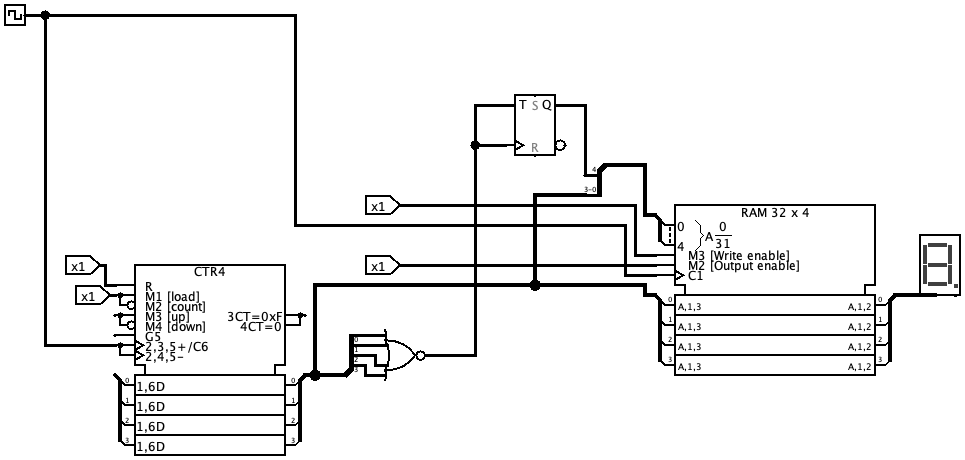
\includegraphics[width=0.3\textwidth]{memory_writer.png}
    \caption{Schematic of Part 1.}
    \label{f:part1}
\end{figure}

    \item Test your modules with \emph{Poke} and the Logisim clock to verify its correctness. Include a few screenshots that shows the contents of the memory unit during your simulation.

\begin{figure}[ht!]
    \centering
    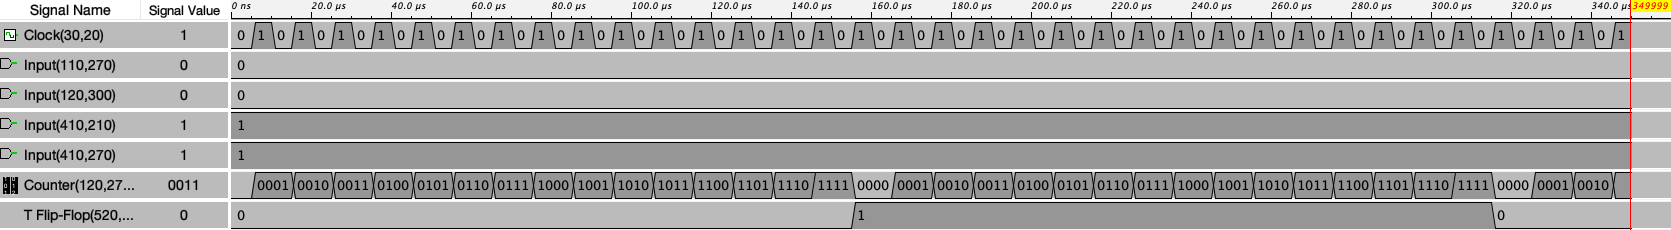
\includegraphics[width=0.65\textwidth]{lab7_Memory Simulation.png}
    \caption{A simulation of the Memory.}
    \label{f:part1_simulation}
\end{figure}

\begin{figure}[ht!]
    \centering
    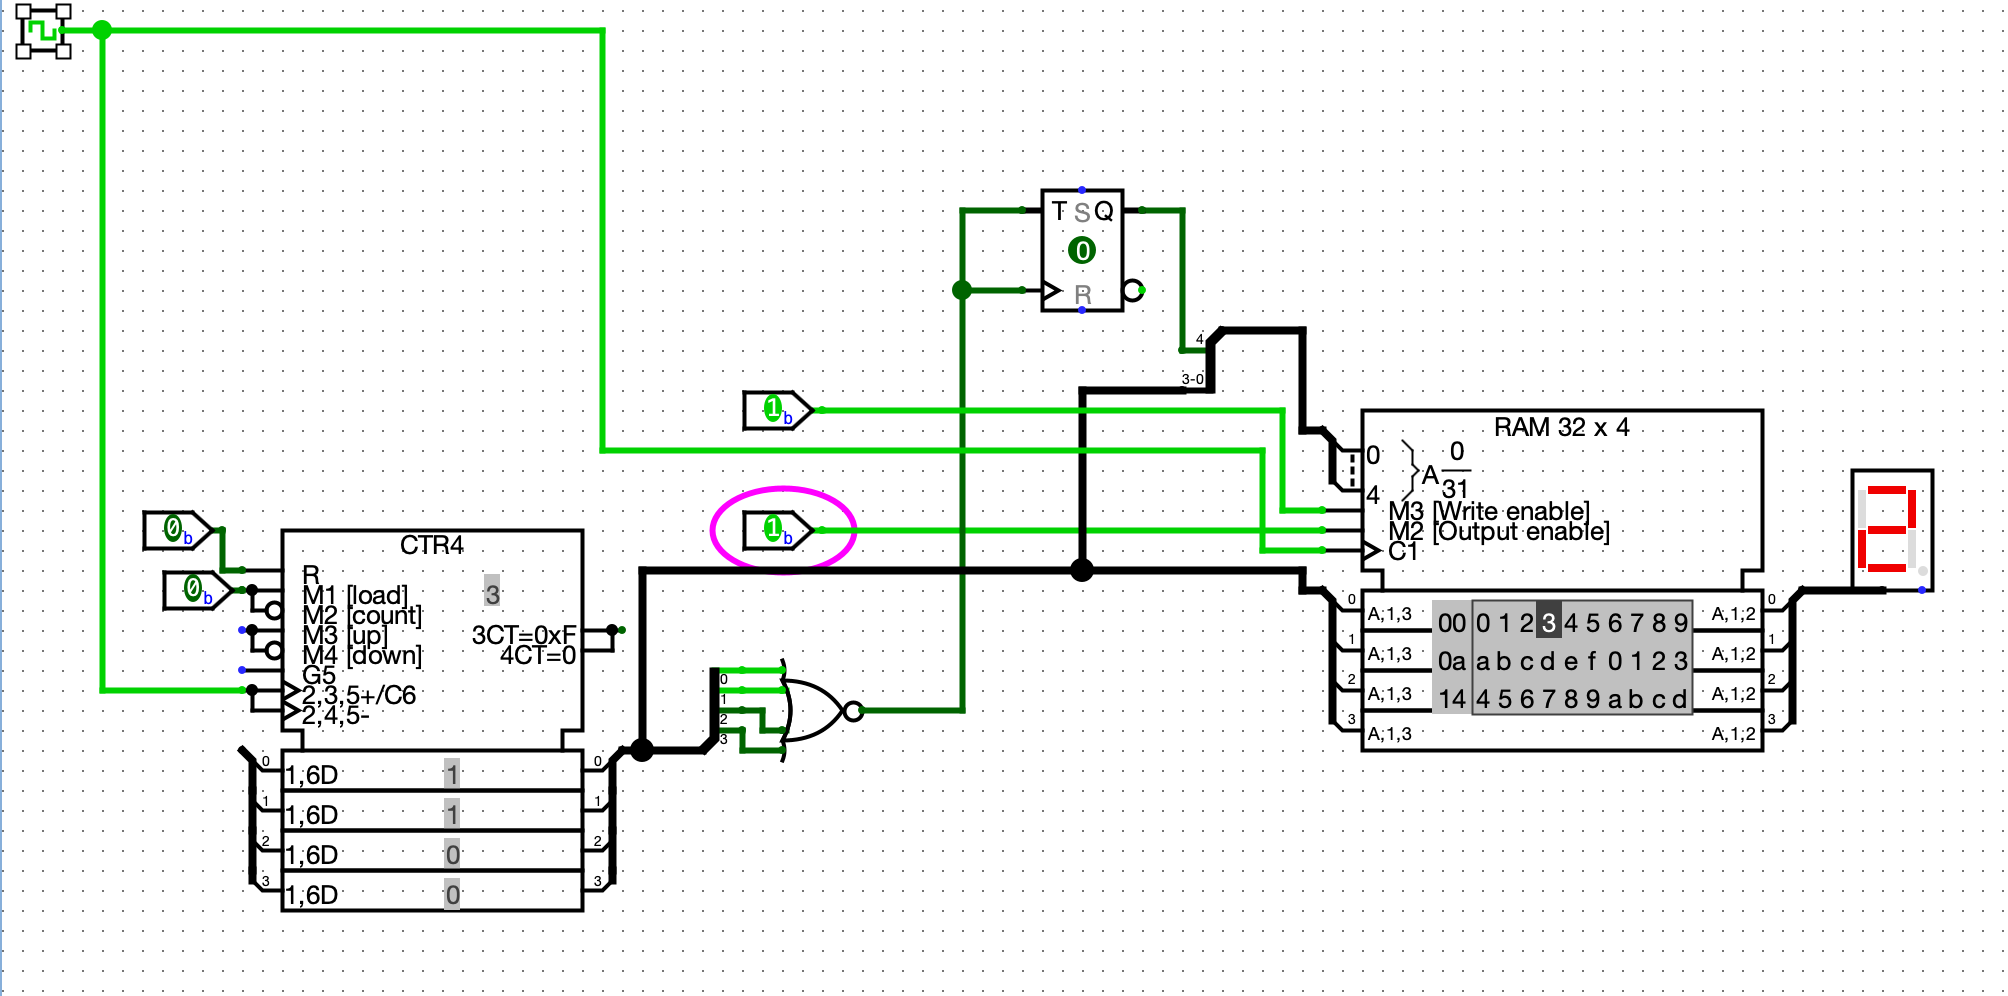
\includegraphics[width=0.65\textwidth]{lab7_Memory Simulation2.png}
    \caption{A simulation of the Memory part 2.}
    \label{f:part1_simulation}
\end{figure}

\end{enumerate}
\newpage
\section{Part II}

% In your report, include the answers to the asked questions, schematics, timing simulations, and test vectors used in your design.
% What you choose to include will vary, but you should use earlier labs as a guide for what is likely important.
% In the end, you will need to be able to describe how your design can draw a square to your TA.
% Think carefully about which figures, tables, and Boolean equations would help in that explanation.
\begin{itemize}

\item What happens if you don’t turn Enable off before updating X and Y?
The square will break and resume drawing at the new X, Y coordinate with some offset determined by the counters in the datapath.
\item What happens if you turn Enable off before 256 clock cycles have passed?
The square will be completed and no new changes will be made. The counters will still cycle through each (X, Y) coordinate in the 16x16 square.
\item What happens if you turn Reset on while Enable is on?
While enable and reset are on, the first pixel at the (X, Y) coordinate will keep attempting to change colour when the clock is high and the counters will not cycle through the indices.

\end{itemize}

\begin{figure}[ht!]
    \centering
    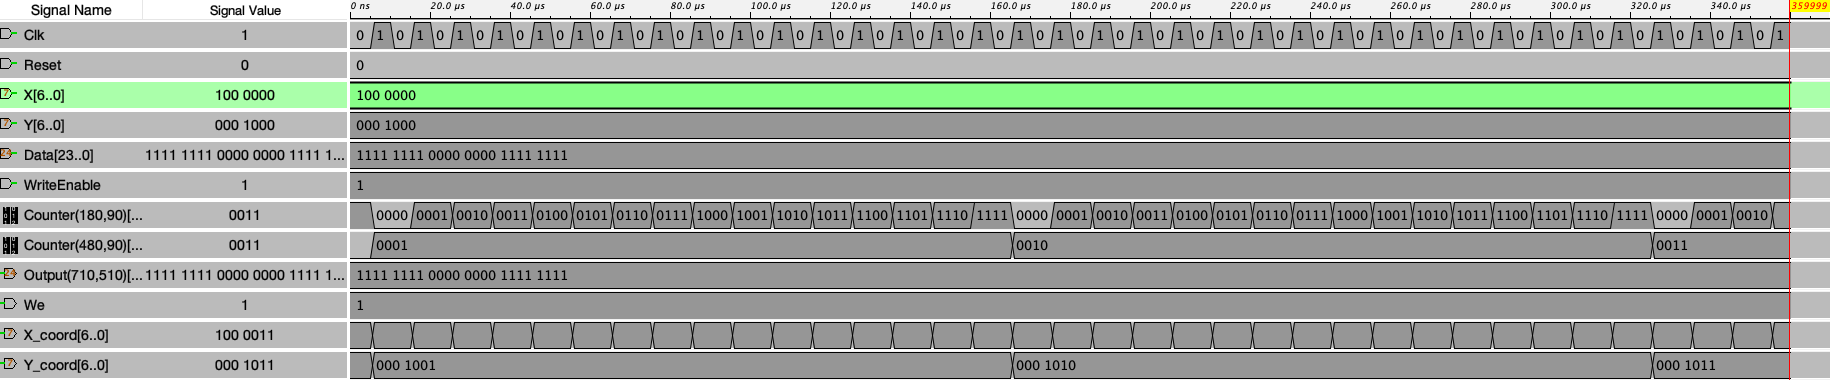
\includegraphics[width=0.65\textwidth]{datapath_timing.png}
    \caption{A simulation of datapath.}
    \label{f:part1_simulation}
\end{figure}

\begin{figure}[ht!]
    \centering
    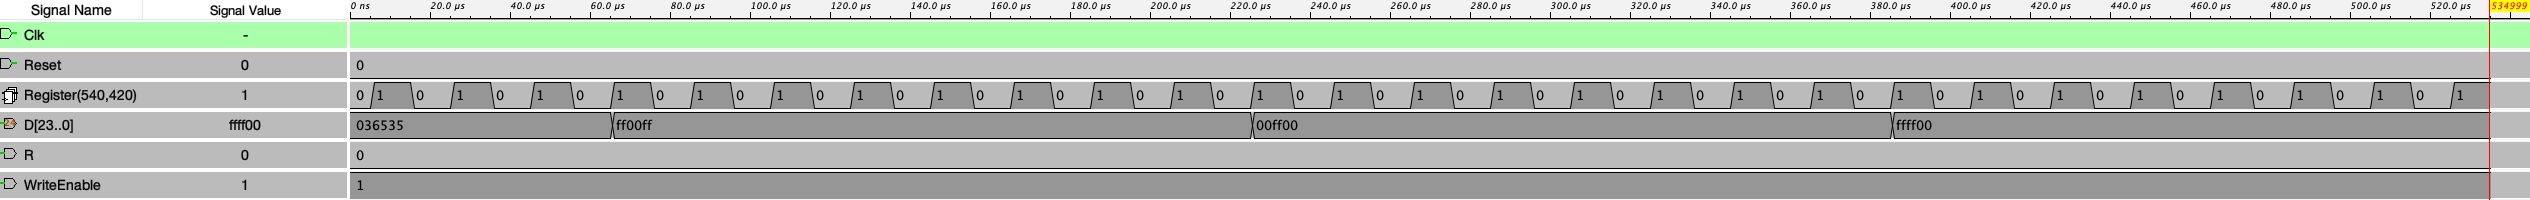
\includegraphics[width=0.65\textwidth]{part2_control_timing.png}
    \caption{A simulation of controlunit.}
    \label{f:part1_simulation}
\end{figure}

\begin{figure}[ht!]
    \centering
    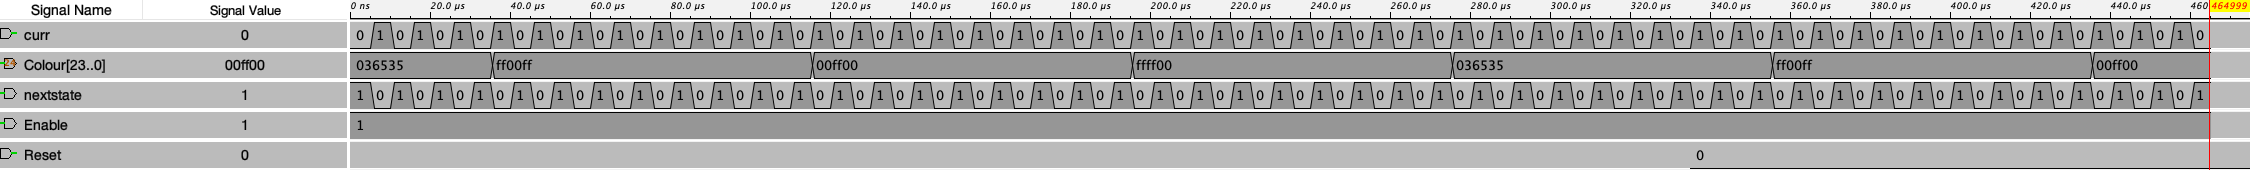
\includegraphics[width=0.65\textwidth]{part2_state_table_timing.png}
    \caption{A simulation of statetable.}
    \label{f:part1_simulation}
\end{figure}



\section{Part III (Bonus)}

\end{document}